\subsection{Class-balanced correctness, retention, and selected-set overlap}
\label{sec:r4-composition-results}
The class-specific results explain how high selected-subset accuracy can coexist with predictions concentrated in a few classes. Table~\ref{tab:r4-composition} and Figure~\ref{fig:r4-composition} compare equal-class correctness and retention at the same coverage as Table~\ref{tab:r3-selectors}. On MNIST at $t=s_C/2$, the certificate's selected-class macro accuracy is 11.24\%, compared with 44.74\% for gated-distance selection. Their macro accepted recalls are 9.88\% and 12.68\%. At $t=s_C$, both selectors retain the same queries and predict class 1 exclusively: selected-class macro accuracy is 10\% and macro accepted recall is 9.79\%. All ten true classes remain represented in these certified subsets, so the 10\% value is the mean of one class with 100\% selected accuracy and nine classes with zero selected accuracy.

\begin{table}[!htbp]
\centering\small
\caption{Composition at the same coverage as Table~\ref{tab:r3-selectors}. Selected-class accuracy gives equal weight to each true class represented in the selected set; accepted recall uses all ten full evaluation classes. Entries are five-seed means $\pm$ sample SD. Jaccard compares the two selectors within each seed.}
\label{tab:r4-composition}
\begin{tabular}{@{}lrrrr@{}}
\toprule
 & \multicolumn{2}{c}{MNIST} & \multicolumn{2}{c}{Fashion-MNIST}\\
\cmidrule(lr){2-3}\cmidrule(lr){4-5}
Measure / selector & $s_C/2$ & $s_C$ & $s_C/2$ & $s_C$\\
\midrule
\multicolumn{5}{@{}l}{Selected-class accuracy (\%)}\\
Certificate & $11.24\pm1.85$ & $10.00\pm0.00$ & $53.36\pm4.76$ & $25.49\pm5.45$\\
Gated distance & $44.74\pm14.35$ & $10.00\pm0.00$ & $63.64\pm7.69$ & $44.21\pm6.17$\\
\multicolumn{5}{@{}l}{Macro accepted recall (\%)}\\
Certificate & $9.88\pm0.17$ & $9.79\pm0.15$ & $30.08\pm2.88$ & $9.63\pm1.44$\\
Gated distance & $12.68\pm0.62$ & $9.79\pm0.15$ & $31.68\pm2.76$ & $12.40\pm2.37$\\
\multicolumn{5}{@{}l}{Effective predicted classes}\\
Certificate & $1.03\pm0.05$ & $1.00\pm0.00$ & $5.35\pm0.90$ & $1.71\pm0.32$\\
Gated distance & $2.14\pm0.43$ & $1.00\pm0.00$ & $6.43\pm0.92$ & $3.73\pm0.77$\\
\midrule
Jaccard & $0.65\pm0.09$ & $1.00\pm0.00$ & $0.70\pm0.07$ & $0.31\pm0.11$\\
\bottomrule
\end{tabular}
\end{table}


For Fashion-MNIST at $t=s_C/2$, selected-class macro accuracy is 53.36\% under certification and 63.64\% under gated-distance selection; at $t=s_C$, it is 25.49\% and 44.21\%. The latter sets have mean Jaccard 0.313 at identical coverage. The effective predicted-class count rises from 1.71 to 3.73 under gated-distance selection, and macro accepted recall rises from 9.63\% to 12.40\%. Thus the stronger baseline accepts a different group of queries and distributes its correct accepted predictions across more classes. The supplement retains each seed's true-class retention, selected-class accuracy, accepted recall, and selected-set overlap, including absent selected classes.

\begin{figure}[!htbp]
\centering
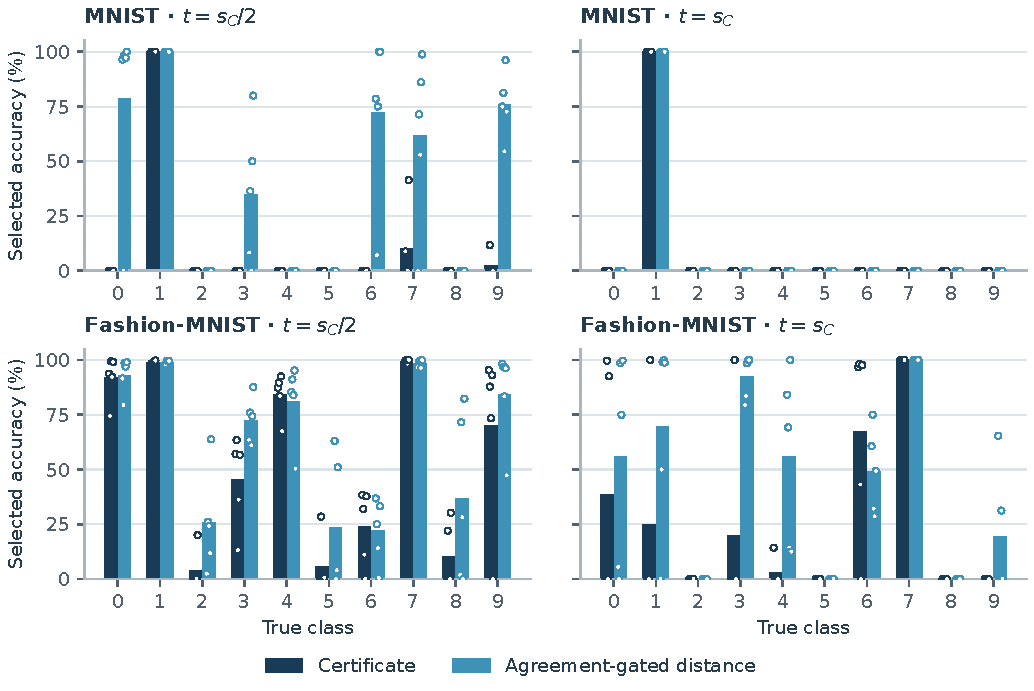
\includegraphics[width=\textwidth]{Figure_07_Selected_Class_Accuracy.pdf}
\caption{Class-specific accuracy within the matched subsets at $\lambda=10\norm{A_t}_2$, using the certificate for $[0.99t,t]$ and the agreement-gated distance comparator. Bars give the five-seed mean selected-class accuracy; hollow points show individual seeds. A class absent from one selected subset has undefined selected accuracy and contributes no point or value to that class's mean. All ten true classes are represented in every MNIST certificate subset. The constant class-1 MNIST endpoint at $t=s_C$ yields 100\% selected accuracy for class 1 and zero for each other represented class. The corresponding class-retention and accepted-recall plots are supplied in the numerical supplement.}
\label{fig:r4-composition}
\end{figure}

\subsection{Observed disagreement and returns along the penalty path}
\label{sec:r4-path-results}
Nearest-prototype agreement is nonmonotone along the sampled regularization paths. Table~\ref{tab:r4-paths} reports the complete grid. A later sampled penalty restores strict agreement in 4.02--6.02\% of MNIST paths and 5.39--6.40\% of Fashion-MNIST paths, depending on prototype budget. Across all groups, 190,405 of 3,366,480 audited query--width paths return to strict agreement after an earlier disagreement. The largest observed number of sign changes is five across the six penalties. For example, Fashion-MNIST seed 22 with $K=100$, width $1.5s_C$, and query 50 alternates between strict agreement and disagreement at every sampled penalty; its competing-minus-reference margins are approximately $-0.017925$, $0.040578$, $-0.033922$, $0.009067$, $-0.017918$, and $0.011859$. Every margin in the exhaustive grid lies outside the numerical guard.

\begin{table}[!htbp]
\centering\small
\caption{Strict disagreement along the six sampled penalties $0,1,10,100,1000,10000$. Percentages are five-seed means $\pm$ sample SD across all 16 widths. Each seed contributes 64,432 query--width paths on MNIST or 160,000 on Fashion-MNIST. Initial disagreement and first detection after zero partition the any-disagreement column. Return denotes a later strict agreement after a sampled disagreement.}
\label{tab:r4-paths}
\begin{tabular}{@{}llrrrr@{}}
\toprule
Dataset & $K$ & Any (\%) & At zero (\%) & First later (\%) & Return (\%)\\
\midrule
MNIST & 50 & $31.20\pm1.26$ & $13.74\pm1.60$ & $17.47\pm0.72$ & $6.02\pm0.94$\\
MNIST & 100 & $27.73\pm1.20$ & $11.18\pm0.86$ & $16.55\pm0.49$ & $4.87\pm0.65$\\
MNIST & 200 & $25.16\pm0.89$ & $8.81\pm1.02$ & $16.34\pm0.61$ & $4.02\pm0.44$\\
Fashion-MNIST & 50 & $25.36\pm2.22$ & $15.46\pm2.57$ & $9.90\pm1.68$ & $6.40\pm1.59$\\
Fashion-MNIST & 100 & $24.85\pm1.36$ & $13.74\pm1.93$ & $11.10\pm1.18$ & $6.01\pm0.95$\\
Fashion-MNIST & 200 & $23.45\pm0.72$ & $12.06\pm0.67$ & $11.40\pm0.36$ & $5.39\pm0.58$\\
\bottomrule
\end{tabular}
\end{table}


The sufficient reversal bound and the first sampled disagreement describe different parts of these paths. At $t=s_C$, all 16,755 finite MNIST bounds and 33,135 finite Fashion-MNIST bounds exceed 10,000. Within those records, 9,714 and 19,154 respectively already disagree at a sampled smaller penalty. A further 878 MNIST and 8,808 Fashion-MNIST records show finite disagreement without a strict limiting reversal at that endpoint. At $t=s_C/2$, all 10,335 MNIST and 5,728 Fashion-MNIST sampled query--penalty pairs above their finite sufficient bounds have positive competing margins. Thus the tail guarantee, sampled onset, and sampled returns are separately recoverable from the same archived family.

\subsection{Coverage at validation-competitive operating points}
\label{sec:r4-competitive-results}
Every validation-competitive archived model has zero sharp full-width certificate coverage. The primary 95\% rule retains 328 models across all 30 groups; the 90\% and 99\% rules retain 494 and 116, respectively, with the same zero-coverage result. Table~\ref{tab:r4-competitive} reports the best-validation choice in each group. All 30 select zero penalty, with widths between $0.75s_C$ and $2s_C$. Evaluation accuracy rises from 82.92\% to 91.80\% across the three MNIST budgets and from 76.23\% to 82.13\% on Fashion-MNIST. The requested full-width regions are excluded for 77.30--98.23\% of Fashion-MNIST queries and 87.53--88.24\% of MNIST queries. These exclusions identify the fraction whose nearest-prototype label fails somewhere inside the family attached to the selected operating point.

\begin{table}[!htbp]
\centering\small
\caption{Validation-selected archived models across all 30 groups. Entries are five-seed means $\pm$ sample SD with the full evaluation set as denominator. All selected models use $\lambda=0$ and have zero sharp full-width coverage. Exclusion concerns the requested region $(0,\sigma]\times[\lambda,\infty)$ attached to the selected endpoint.}
\label{tab:r4-competitive}
\begin{tabular}{@{}llrrr@{}}
\toprule
Dataset & $K$ & Accuracy (\%) & Nearest agreement (\%) & Region excluded (\%)\\
\midrule
MNIST & 50 & $82.92\pm0.46$ & $65.75\pm5.37$ & $87.53\pm0.28$\\
MNIST & 100 & $88.43\pm0.27$ & $73.94\pm2.43$ & $88.07\pm0.14$\\
MNIST & 200 & $91.80\pm0.31$ & $79.83\pm2.52$ & $88.24\pm0.14$\\
Fashion-MNIST & 50 & $76.23\pm0.88$ & $62.72\pm4.74$ & $98.23\pm3.13$\\
Fashion-MNIST & 100 & $79.38\pm0.63$ & $68.35\pm4.02$ & $93.75\pm8.61$\\
Fashion-MNIST & 200 & $82.13\pm0.19$ & $73.58\pm1.69$ & $77.30\pm4.81$\\
\bottomrule
\end{tabular}
\end{table}


Increasing prototype budget improves the evaluation accuracy of the validation-selected readout at each budget step in every seed of both datasets. The paired $K=50$ to $K=200$ gain is $8.88\pm0.41$ percentage points on MNIST and $5.90\pm0.80$ on Fashion-MNIST. Across the ten seed pairs, mean prediction disagreement falls from 14.29\% to 5.95\% on MNIST and from 12.21\% to 8.15\% on Fashion-MNIST. Mean Jaccard overlap of correctly classified queries rises from 0.874 to 0.947 and from 0.885 to 0.922, respectively. The supplement retains every paired value, all class counts, and accuracy--coverage plots for all 2,880 readouts.

\subsection{Accumulation of exclusions under a fixed finite-probe order}
\label{sec:r4-probe-results}
Expanded finite probes recover most original limiting-witness cases early in the recorded sequence. At $t=s_C$ and floor zero, $F_1$ reaches 95\% of $L_0$ after mean 15.6 MNIST and 20.2 Fashion-MNIST checks, in all five seeds (Table~\ref{tab:r4-probes}). The original finite set $F_0$ never reaches this target in these ten groups. All $L_0$ cases are recovered by $F_1$ on MNIST after mean 17.6 checks. On Fashion-MNIST, $L_0$ retains a unique set comprising 0.134\% of all queries after the full expanded sequence. The final $F_1$ finite exclusion set is recovered after mean 49.6 of 100.8 eligible checks on MNIST and 107.4 of 107.4 on Fashion-MNIST. The stored step records identify which additional widths and penalties supply each increment.

\begin{table}[!htbp]
\centering\small
\caption{Fixed-order accumulation at $t=s_C$ and penalty floor zero. Checks are archived readout evaluations in the recorded round-robin order. The recovery target is 95\% of the original limiting-witness set $L_0$ within each seed. Means use five seeds; a dash means the target was not reached. The final column has the full query population as denominator.}
\label{tab:r4-probes}
\begin{tabular}{@{}llrrrr@{}}
\toprule
Dataset & Set & Eligible checks & Reaching target & Checks to target & $L_0$ unique (\%)\\
\midrule
MNIST & F0 & 84.0 & 0/5 & --- & 8.026\\
MNIST & F1 & 100.8 & 5/5 & 15.6 & 0.000\\
Fashion-MNIST & F0 & 84.0 & 0/5 & --- & 21.458\\
Fashion-MNIST & F1 & 107.4 & 5/5 & 20.2 & 0.134\\
\bottomrule
\end{tabular}
\end{table}

